\documentclass[12pt]{report}
\usepackage[style=ieee]{biblatex}
\addbibresource{references.bib}
\usepackage{enumitem}
\setlist[enumerate]{nosep}
\usepackage{fancyhdr}
\usepackage{float}
\usepackage{fontspec}
\usepackage[letterpaper,hmargin={47.5mm,17.5mm},top=64.0mm,bottom=25.4mm]{geometry}
\usepackage{indentfirst}
\usepackage{microtype}
\usepackage{multirow}
\usepackage{setspace}
\usepackage{tabularx}
\usepackage[explicit]{titlesec}
\usepackage{tocbibind}
\usepackage{wallpaper}

\newcommand{\authora}{
    Basil Eric C. Rabi %
}
\newcommand{\authorb}{
    James M. Paje %
}
\newcommand{\authorc}{
    John Kenneth C. Velonta %
}
\newcommand{\authord}{
    Richard Banog %
}
\newcommand{\eg}{\emph{e.g.}}
\newcommand{\hypothesis}[1]{
\noindent \textbf{Research Question:}

Is there a significant difference between the existing monitoring system and the real-time monitoring system in terms of #1?

\begin{quotation}
    \noindent \textbf{Null Hypothesis ($H_o$)}:
    
    There is no significant difference between the existing monitoring system and the real-time monitoring system in terms of #1.

    \noindent \textbf{Alternative Hypothesis ($H_a$)}:
    
    There is a significant difference between the existing monitoring system and the real-time monitoring system in terms of #1.
\end{quotation}

}

\newcommand{\thetitle}{SAFER: Design of a Real-Time Equipment Monitoring System Using Integrated GSM-GNSS Modules}

%Alternate Titles:
%SAFER: An IoT Integrated Real-Time Equipment Efficiency Monitoring for Surface Mines
%SAFER: Design of a Real-Time Equipment Monitoring System Using Integrated GSM-GNSS Modules

\usepackage[hidelinks]{hyperref}
\hypersetup{
    pdfborder  = {0 0 0},
    pdfinfo    = {
        Title    = {\thetitle},
        Subject  = {Internet of Things},
        Author   = {\authora and \authorb and \authorc and \authord},
        Keywords = {IoT, Mining, Equipment, GSM, GNSS}
    }
}
\usepackage[section]{glossaries}
\makeglossaries

\newglossaryentry{c}{
    name=C,
    description={A high-level general-purpose programming language. Programs written in this language needs to be compiled but can be optimized based on targetted hardware}
}
\newglossaryentry{gammu}{
    name=gammu,
    description={A programming library to easily interface with GSM devices \cite{gammu}}
}
\newglossaryentry{gnss}{
    name=GNSS,
    description={Global Navigation Satellite System.
        A navigation system which provides autonomous geo-spatial positioning on a global coverage.
        This uses satellite constellations such as GPS (USA), GLONASS (Russia), Beidou (China), Galileo (EU), INRSS (India) and QZSS (Japan) \cite{GNSS}}
}
\newglossaryentry{gsm}{
    name=GSM,
    description={Global System for Mobile Communication.
        A wireless communication system which enables exchanging of Short Message Service (SMS) text messages between mobile devices \cite{GSM}}
}
\newglossaryentry{gtk}{
    name=GTK,
    description={An open-source library used for creating graphical user interface \cite{gtk}}
}
\newglossaryentry{heavyequipment}{
    name=Heavy Equipment,
    description={Machineries used in mining operations that are mostly utilized in the loading of ores.
    Compared to light equipment, heavy equipment are mostly static in location.}
}
\newglossaryentry{iot}{
    name=Internet of Things (IoT),
    description={A network of electronic devices with seamless communication with each other \cite{IoT}}
}
\newglossaryentry{microplastics}{
    name=microplastics,
    description={Plastic particles with sizes of less than 5 millimeters \cite{Microplastic}}
}
\newglossaryentry{pms}{
    name=PMS,
    description={Preventive Maintenance Schedule.
        This is a program designed to prevent equipment breakdowns and extend the lifespan of equipment through regular maintenance activities such as inspections, cleaning, lubrication, and replacement of worn or damaged parts.
        The schedule is based on the manufacturer's recommendations, operating conditions, and equipment usage}
}
\newglossaryentry{postgis}{
    name=PostGIS,
    description={An extension of PostgreSQL which allows storing and processing geo-spatial data such as points, line strings and polygons \cite{postgis}}
}
\newglossaryentry{postgres}{
    name=PostgreSQL,
    description={An SQL-compliant open-source relational database management system \cite{postgres}}
}
\newglossaryentry{python}{
    name=python,
    description={A modern interpreted general-purpose programming language.
        Unlike C, programs written in this language do not require compilation and are easier to read and debug}
}
\newglossaryentry{rpi}{
    name={Raspberry Pi},
    description={A low-cost single-board computer with a processor similar to smart phones}
}
\newglossaryentry{smr}{
    name=SMR,
    description={Service Meter Run.
        Number of hours or kilometers that the equipment has operated}
}
\newglossaryentry{database}{
    name={Relational Database},
    description={A collection of tabular data wherein one table can be related to one or more tables}
}
\newglossaryentry{sql}{
    name=SQL,
    description={Structured Query Language.
        This is used in programming and managing data stored in a relational database management system}
}
\newglossaryentry{tmc}{
    name=TMC,
    description={Taganito Mining Corporation.
        A mining company operating a surface mine situated in Tagantio, Claver, Surigao del Norte, Philippines}
}

\addtolength{\headwidth}{15pt}
\doublespacing
\renewcommand{\contentsname}{TABLE OF CONTENTS}
\renewcommand{\headrulewidth}{0pt}
\setmainfont[Mapping=tex-text-ms]{Times New Roman}
\setlength{\headheight}{15pt}
\setlength{\parindent}{12.7mm}
\setcounter{secnumdepth}{3}
\titleformat{\chapter}[block]{\bfseries\centering}{}{0em}{#1}
\titlespacing{\chapter}{0pt}{-20pt}{30pt}

\begin{document}

\ULCornerWallPaper{1}{spus.pdf}
\pagenumbering{roman}
\addcontentsline{toc}{chapter}{TITLE PAGE}
\thispagestyle{empty}

\begin{center}

\vspace*{1cm}
\textbf{\MakeUppercase{\thetitle}}

\vspace{1.5cm}
A Research Concept Paper Presented to \\
The College of Engineering \\
St. Paul University Surigao

\vfill

In Partial Fulfillment of the Requirements for the Course \\
RESEARCH METHODS

\vspace{1cm}
By:

\vspace{1cm}
\textbf{\authora} \\
\textbf{\authorb} \\
\textbf{\authorc} \\
\textbf{\authord} \\

\vspace{1cm}
March 2023

\end{center}

\fancypagestyle{plain}{
    \fancyhead{}
    \fancyfoot{}
    \fancyhead[R]{\thepage}
}

\pagestyle{fancy}
\fancyhead{}
\fancyfoot{}
\fancyhead[R]{\thepage}

\tableofcontents

\titleformat{\chapter}[block]{\bfseries\centering}{CHAPTER \thechapter\\#1}{0em}{}
\titleformat{\section}[block]{\bfseries\centering}{\MakeUppercase{#1}}{0em}{}
\titleformat{\subsection}[block]{\bfseries}{#1}{0em}{}
\titleformat{\subsubsection}[block]{}{\emph{#1}}{0em}{}

\chapter{THE PROBLEM AND ITS BACKGROUND}

\pagenumbering{arabic}

\section{Introduction}

\subsection{Environmental Impacts of Equipment in Surface Mines}

Heavy equipment and machinery are essential in large scale surface mine operations in order to have an acceptable amount of throughput.
However, usage of such tools in surface mines have significant impacts to the environment.
Theses impacts include greenhouse gas emissions, consumption of non-renewable resources from fuel and equipment parts, dust generation, and accident risks.
The only way to minimize this impact is to use heavy equipment efficiently.

\subsubsection{Fuel Consumption and Greenhouse Gas Emissions}

Heavy equipment and machinery contribute significantly to greenhouse gas emissions due to their high fuel consumption.
Based on the available data from a surface mine in the Philippines, heavy equipment consumes 9-25 liters of diesel fuel per hour depending on the model.
The worldwide sales of such equipment amount to one million units annually, making it imperative to address this issue \cite{EquipmentFuelOptimization}.
Furthermore, the inefficient use of these machines only exacerbates the problem.

Idling equipment units are a significant cause of increased fuel consumption in surface mines.
Additionally, a mismatch in the loader-to-hauler ratio can further reduce fuel efficiency.
If the number of haulers is too high, queuing can lead to an increase in fuel consumption per ton moved.
Conversely, if there are too few haulers, the loading unit will idle, leading to an increase in fuel consumption per ton moved.

Real-time data can be utilized to effectively reduce fuel consumption by identifying idling units and addressing the loader-to-hauler equipment ratio promptly.
By doing so, fuel consumption can be reduced, and greenhouse gas emissions can be lowered.

\subsubsection{Dust Generation and Accident Risk}

Studies have shown that hauling speed is strongly correlated with both dust generation and the risk of accidents.
Higher speeds can lead to increased dust concentrations \cite{SpeedDust}, as well as an increase in both the frequency and severity of accidents \cite{SpeedAccident}.

Unsafe driving practices such as overtaking along intersections and curves, and over-speeding violate rule 414 of DENR Administrative Order 2000-98 \cite{DAO2000-98}.
It is essential to take proactive measures to detect and control such violations.
By utilizing real-time data, haulers violating the speed limit can be identified and corrected promptly.

Implementing measures to control speed violations can have a significant impact on reducing dust generation and improving safety performance.
Compliance with Philippine Mine Safety Regulations can also be ensured through this approach.
By taking proactive measures, we can reduce the risk of accidents, promote a safer work environment, and reduce the negative impact of dust generation on health and the environment.

\subsubsection{Solid Waste Generation from Tires and Paper Usage}

Solid waste generation from tire wear and paper usage are two environmental issues that are prevalent in the mining industry.
Higher speeds are known to cause increased tire wear \cite{TyreWear}, which in turn generates more waste from used tires.
Furthermore, tire wear contributes to the generation of \gls{microplastics}, which are a widespread pollutant in marine environments \cite{TireMicroplastic}.
One way to minimize waste generation, including microplastics, is to control the speed of wheeled equipment.

In the Philippines, surface mines collect equipment monitoring data using paper-based forms.
This practice requires each operator to fill out a two-page form summarizing their equipment usage during their shift. 
With this system in place, a surface mine with 500 equipment units can consume a ton of paper in less than three months. 
However, the paper industry is known to cause several environmental issues, such as deforestation, greenhouse gas emissions, and water pollution \cite{PaperIndustry}.

One solution to these issues is to implement a paperless and real-time monitoring system for equipment usage.
This system would reduce solid waste generation from tires and eliminate the need for paper usage.
By using digital forms, surface mines can significantly reduce their environmental impact and promote sustainability.

\subsection{Real-time Data Collection and IoT}

Data is the life-blood of any company, regardless of which industry this may come from, as it provides vital insights that can help in making informed decisions.
Due to the sheer volume of industrial data that could be extracted at any given time, it is often a big undertaking to even attempt to make a data pipeline that is scalable to the highly defining characteristics of industrial data; high dimensionality and process dynamics, and large yet redundant \cite{Urhan}.

The mining industry is no exception when it comes to large amount of industrial data prime for extraction.
For example, mining companies, whether surface operations or otherwise, utilize large fleets of equipment for various purposes.
This alone can generate thousands, if not millions of rows of real-time data per day depending on the parameters that the company decides to obtain from these equipment.
The advent of using information technologies in big industries have led authors to coining different terminologies such as \textit{Smart Mining}, \textit{Industry 4.0}, and \textit{Digital Revolution} among others \cite{SmartMining}.

One emerging technology that has the potential to revolutionize the mining industry is the Internet of Things (\Gls{iot}).
IoT is a concept that enables seamless communication between electronic devices and is already widely used in various fields such as environmental monitoring, healthcare, and transportation \cite{IoT}.
By leveraging IoT, real-time information can be gathered and companies can improve the reliability of their data collection by automating tasks and minimizing human errors.
Access to real-time information also allows making decisions and taking actions in a more prompt manner.

IoT is now being used in mining companies worldwide to promote sustainability, improve safety, and enhance productivity \cite{IoTinMining}.
In the Philippines, an IoT system called ER MineTracer was recently designed to improve emergency response during an incident in a mine by replacing manual communication of location via handheld radios with more reliable devices such as GPS units and mobile phones \cite{ERMineTracer}.

One example from the international landscape is the Koodaideri Iron Ore Mine in Pilbara, Western Australia, a project of the Rio Tinto Group.
In 2018, the Rio Tinto Group announced its plans to build 'intelligent mine' for its Koodaideri project\cite{koodaideri1}.
In 2019, the group declared its partnership with the machineries manufacturer, Caterpillar, and exclusively purchased equipment from the manufacturer with agreement to study the potential of increased automation in Koodaideri project\cite{koodaideri2}.
In 2021, Rio Tinto Group officially launched its Safe Production System (SPS) as a way to improve their operation through automated data collection\cite{sps}, a culmination of their years of effort to build an 'intelligent mine'.
In this specific instance however, the Koodaideri Project is exclusively served by Caterpillar and its proprietary systems.
While the technology is already available, most commercially present systems are vendor-locked to the equipment manufacturer.
In the case of most mining operations in the country, this would be less beneficial and less cost-effective as most of the companies purchase different types of equipment from different manufacturers.
Thus the need for a low-cost, manufacturer agnostic system to automatically monitor and collect data is a challenge that if addressed, would be very beneficial to the host company.

\subsection{Present Challenges in Philippine Surface Mines}

In Philippine surface mines, equipment usage data is still manually collected using paper-based forms, leading to several operational challenges discussed below.

\subsubsection{Inadequate Operational Control}

The current manual data gathering method provides inadequate operational control, as any inefficiency can only be detected and quantified after a month of data collection.
This delay makes it difficult to detect occurrences of idling equipment and sub-optimal loader-to-hauler ratios in equipment deployment, which increases resource consumption.

\subsubsection{Weak Enforcement of Speed Limit}

Speed limits are imposed in all surface mines to lessen risks of accidents and to control dust generation.
However, enforcement of the speed limit is only done thru verbal instructions and violations can only be detected through random checks by safety inspectors.
This results in a low detection rate of over-speeding vehicles.

\subsubsection{Low Data Integrity}

The current paper-based data collection method is prone to human error, which affects data integrity.
The forms are initially filled-out by operators, manually checked by supervisors, and signed-off by foremen after an 8- to 12-hour shift.
The filled-out forms are then encoded in a spreadsheet the next day, and data consolidation and review are done on a monthly basis.
Human errors can be introduced twice during this process: during filling-out and during encoding.
Erroneous data are not completely detected and corrected since spreadsheet-encoded data can only be checked manually. 
Furthermore, the mine operations team and the equipment maintenance team monitor equipment usage separately, often resulting in contradicting information.

\subsubsection{Early Equipment Downtime}

When an equipment breakdown occurs, repairing the down unit can be delayed from 1 shift up to several days if the breakdown is not promptly relayed to the maintenance crew, or if the maintenance crew is unable to pinpoint the exact location of the down unit during their deployment.
Moreover, equipment servicing is done at fixed intervals of usage (\eg 500 hours) as part of the equipment preventive maintenance program.
However, actual usage of the equipment prior to servicing often exceeds this duration since equipment usage data is finalized monthly.
This poor implementation of the maintenance program leads to early downtime of equipment \cite{EquipmentProductivity}.

\section{Conceptual Framework of the Study}

This study uses a similar IoT system in a research study of a home security system which used a GSM module and a \Gls{rpi} \cite{GSMRPi}.
There will be four major milestones in the development cycle of the study as illustrated in Figure~\ref{fig:development_cycle}.

\begin{figure}[H]
    \centering
    \includegraphics[clip, trim=97mm 2mm 2mm 33mm, width=\linewidth]{img/development_cycle.pdf}
    \caption{Development cycle of the real-time equipment activity monitoring system using GSM-GNSS module.}
    \label{fig:development_cycle}
\end{figure}

Each part of the development cycle shall be discussed in the succeeding chapter in full capacity. 
But the basic premise of the framework is first to identify the data and feature requirements to be included in the study.
Next is building a system design based upon the identified requirements, then the evaluation of the built system and a process loop based on the feedback of the end-users.
And then lastly, evaluation of the impact of the final system produced by the researchers.

\section{Statement of the Problem}

This study aims to develop real-time monitoring and control system for equipment usage, leveraging IoT technology, which can lead to improved operational efficiency, stronger enforcement of speed limits, higher data integrity, and decreased equipment downtime in Philippine surface mines.
Throughout the duration of this study, the following questions will be addressed:

\begin{enumerate}
    \item How efficient is the current data collection and processing system of the host surface mining company in terms of
        \begin{enumerate}
            \item Turn-over time of data from Mine Division to Finance Department
            \item Gap between the actual \Gls{smr} during actual \Gls{pms} and the pre-defined SMR requiremment for PMS (500 hours for \Gls{heavyequipment} and 5000 km for light equipment)
            % time a = actual 500 smr
            % time b = 500 smr recorded by TSD/PMS
            \item Equipment over-speeding detection
            \item Idling time registry accuracy and detection
            % time a = actual smr between
        \end{enumerate}
    \item How is the system developed in relation to
            \begin{enumerate}
                \item Hardware selection
                \item Software stack selection
                \item Current system used by the company
                \item End-user's requirement and feedback
            \end{enumerate}
    \item How efficient is the researcher's data collection and processing system of the host company in terms of
        \begin{enumerate}
            \item Turn-over time of data from Mine Division to Finance Department
            \item Gap between the actual SMR during actual PMS and the pre-defined SMR requiremment for PMS (500 hours for heavy equipment and 5000 km for light equipment)
            \item Equipment over-speeding detection
            \item Idling time registry accuracy and detection
        \end{enumerate}
    \item What is the significant difference between the presently employed system and the new system?
    \item What is the evaluation of the system by the experts in terms of
        \begin{enumerate}
            \item Efficiency
            \item Stress tolerance
            \item End-user's experience
        \end{enumerate}
\end{enumerate}

\section{Hypothesis}

\hypothesis{turn-over time of data from Mine Division to Finance Department}
\hypothesis{gap between the actual SMR during equipment servicing and the pre-defined SMR requirement for PMS}
\hypothesis{detection rate for over-speeding equipment}
\hypothesis{detection rate for idling equipment}

\section{Significance of the Study}

The objective of the study is to produce a working prototype of a real-time monitoring and control system system for equipment usage.
This study will leverage IoT technology through the use of commercially available \Gls{gsm} and \Gls{gnss} modules removing the need for paper-based forms and manual data encoding, and possibly removing the need for mobile internet data reception to transmit live data to the central server.
This study also makes it possible to create a real-time dashboard and location mapping of equipment which will improve the response time to changes and sub-optimal conditions in the operation.

This study is in-line with the goal of environmental sustainability of the mining industry through the use of modern technology.
The use of the system being proposed in this study will help mining companies control their fleet more efficiently, reducing the fuel consumption caused by idling of equipment due to over or under assignment of trucks within an area.
The proposed system also hosts a feature that alerts over-speeding of trucks, which could reduce the dust generation during the hauling activity and solid waste generation from tire wear. 
The host company could also benefit differently from this feature, as it also alerts the supervisors, safety officers, and managers when over-speeding has occurred, reducing the risk of accidents.

The proposed features of the end-product are listed below, subject to change depending on the feedback of the end-users:
\begin{itemize}
\setlength\itemsep{-0.5em}
    \item Real-time equipment location monitoring
    \item Paperless equipment activity monitoring
    \item Touch-based equipment activity input
    \item Over-speeding detection and notification system
    \item SMS-based data send-out
    \item Web-based front-end for real time data monitoring
    \item Paperless service meter run data collection
    \item Automated Preventive Maintenance Schedule notification system
    \item Assisted correction of data through automation of anomalous data detection
\end{itemize}

The proposed system has the potential to minimize environmental impacts and reduce the risk of vehicular accidents.
With this system in place, mining companies can improve their operations, enhance safety, and promote sustainability.

\section{Scope and Limitation of the Study}

The whole system and product development, testing, data collection, and end-user engagement will be done solely at \Gls{tmc} for the purpose of convenience.
This means that the product's feature design, user interface and user experience choices, and the study's conceptual layout will be based on the operational framework and end-user feedback from TMC alone.
Should the output of this study be applied elsewhere, minor changes will have to be made in order to accommodate the different operational framework of another mining company.

A limiting factor that may affect the degree of real time data collection process is the SMS network reception of a given area.
The researchers will be addressing this issue and provide a solution so that the data collected by the device could still be sent at a later time when network reception is available.
The available solutions however, could still reduce the degree of real time data collection.

\newpage
\printglossary[
    type=main,
    nonumberlist,
    numberedsection,
    title={Definition of Terms},
    toctitle={Definition of Terms}
]

\chapter{METHODS}
%Assigned to JK

The researchers shall use the conceptual framework discussed in the previous chapter in the development of the system.
The complete process flow of each major milestone of the research will be discussed in this chapter.
The methods to be used by the researchers will require knowledge on hardware and software components, operational process of the host company, and statistics.

\section{Research Design}

This study aims to design a system composed of substitution of manual data gathering process, writing software components, and integration of hardware components.
Thus the Developmental Research Design will be applied initially.
The performance of the system prototype will be compared with the existing data collection system in a surface mine.
This comparison shall employ a Quantitative-Descriptive Research Design.

\section{Participants}

The participants of this study shall compose of personnel coming from departments or divisions relevant to the chosen company's operation that utilizes heavy and light equipment. 
These would be operators of equipment and their respective supervisors and managers from the the Technical Services Department (TSD) and the Mines Division. 

The TSD personnel are tasked to attach the device to the chosen equipment for the testing of the product.
The operators are tasked to use the product and will be utilizing the built-in software the researchers have installed onto the device.
The supervisors are responsible for the assignment of operators and equipment to the device, the data validation stage, and the real time monitoring of the equipment utilization.
The managers shall observe the overall effects brought about by the product to the efficiency of the day-to-day operation of the company.

\section{Methodology}

The aforementioned milestones that were briefly discussed in the previous chapter's \textit{Conceptual Framework} section will be discussed in full detail in this section.
Each milestone shall represent one major part in the methodology of this research.

\subsection{Formulation of Requirements}

The functionalities and the features of the data collection system will be identified first.
As the research progresses, the functionalities will be illustrated as use-case diagrams which are analogous to the design requirements \cite{UseCase}.
The formulation of requirements will depend upon the existing process and systems implemented by the host company.
The formulation of requirements is a way to identify the gaps in the company's process' efficiency that can be addressed by researcher's propose system.

\subsection{System Design}

Bulk of the work in this study is designing the system.
The system shall address all requirements to be identified in the previous development milestone.
An initial high-level design drafted by the authors is shown in Figure~\ref{fig:concept_structure}.

\begin{figure}[H]
    \centering
    \includegraphics[clip, trim=0 0 0 12mm, width=\linewidth]{img/feature_context.pdf}
    \caption{Conceptual level structure of the equipment usage data collection system.}
    \label{fig:concept_structure}
\end{figure}

\subsubsection{Hardware Selection}

The researchers chose to utilize Raspberry Pi 3B+, a single-board computer (SBC) made by Raspberry Pi Foundation, as the device's processing unit due to its low-cost yet sufficiently capable hardware for the project. 
The low-cost of the computer will help chances of this project to have an increase in production count once a final product is demonstrated.
A 7-inch  touchscreen monitor will be connected to the Raspberry Pi computers which will serve as the display for the graphical user interface, and will be receiving touch input from the operators depending on their current activity.
The researchers will be attaching commercially available integrated GSM-GNSS modules to the devices to act as receiver of location data, and sender of collected data to the central server.
A low-cost voltage regulator will also be utilized in order to control the device's voltage input to 5.1 volts, the official voltage recommendation by the Raspberry Pi Foundation \cite{rpi}, to protect the device from power fluctuations which may harm the device or corrupt the data. 

On the server side, the researchers will be using a USB GSM module that will act as the receiver of the location and equipment utilization data sent by the device attached to the equipment. 
The computer that will act as the central server of the study will be a Lenovo ThinkSystem SR650 which is equipped with the second generation of Intel Xeon Processor Scalable Family (Xeon SP Gen 2).

\subsubsection{Source Code Writing}

The researchers will be using the official Raspberry Pi OS as the operating system for the device.
For the Graphical User Interface (GUI) of the device, the researchers will be using \Gls{gtk}, a free and open-source widget toolkit for creating graphical user interfaces.
The sending of location and equipment utilization is made possible through the use of \Gls{python}-\Gls{gammu}, a library and command line utility for python which can be used to control GSM capable devices. 

On the server side of the system, the server will be running Fedora Linux as its operating system.
The researchers will still be using python-gammu to receive SMS text from the equipment.
The data received will be processed and parsed by the server through Python scripts.
The data will then be stored using \Gls{postgres} extended by \Gls{postgis} as the database management system for the study.

The graphical user interface for the supervisors will be made through Django, a high-level Python web framework, specifically through its Admin and Views features.
QField, a mobile Geographic Information System (GIS) application and QGIS, a desktop GIS application with direct interface to PostgreSQL database, may also be used by the engineers to access and view the real-time data of the equipment 

\subsection{System Testing}

For convenience purpose, the researchers chose to conduct the device's testing in Taganito Mining Corporation (TMC), a nickel mining company operating in Taganito, Claver, Surigao del Norte, Philippines.
TMC is also the workplace of all the aforementioned researchers of this study. 
Prior to the actual device pilot test, a meeting with the managers and personnel of the involved departments shall be conducted to introduce and explain the purpose of this study and the produced hardware. 
All questions about the study shall be addressed by the researchers in the meeting.

After clearance is given by the managers of the concerned departments, the researchers shall request the service of the staff of Technical Services Department for the attachment of the device to the chosen equipment.
Testing will be made, and feedback from the end-users shall be collected and considered for revision of the system.
Revisions will then be applied to the device and software, and testing will be continued, and feedback will be collected once again.
The cycle of testing-feedback-revision will continue until the end-users are satisfied with the experience and functionality brought by the device and the accompanying software.
The data gathering and system evaluation flow can be summarized as follows:

\begin{figure}[H]
    \centering
    \includegraphics[clip, trim= 10mm 55mm 0 5mm, width=0.88\linewidth]{img/Data Gathering procedure1.pdf}
\end{figure}

\begin{figure}[H]
    \centering
    \includegraphics[clip, trim= 10mm 55mm 0 5mm, width=0.88\linewidth]{img/Data Gathering procedure2.pdf}
    \caption{Data gathering and system evaluation process.}
    \label{fig:Data Gathering procedure2.pdf}
\end{figure}

\subsection{Evaluation}
%Assigned to Richard

\subsubsection{Descriptive Statistics}

 The same method of comparison will be used based on the ER Mine Tracer study's research design.
 The researchers of the said study used survey to compare the Walkie-Talkie and ER Mine Tracer's functionality and efficiency.
 This research will also employ surveys to gather data on the users' experience and opinion regarding the researcher's data collection and processing system and compare it to the company's current systems.
The efficiency of the host company's data collection and processing system and the researcher's system will be compared in terms of data turnover time from the Mine Division to the Finance Department, the discrepancy between the actual SMR during the actual PMS and the predefined SMR, and over-speeding detection of the current system and idling equipment accuracy and detection.  
A Likert 4-point scales for "Agreement" parameter with 0.25 point increment will be basis of point system of the questionnaire. For each parameter, the verbal response and qualitative description provided by the system validators are used to generate the scale. Depending on the name of the performance exam, the first scale, or maximum, ranges from 3.25 to 4.00 with a parameter of 4 and a vocal response of "strongly agree".
The second scale has a range of 2.5–3.25, a parameter of 3, an agree verbal response, and a qualitative description based on the name of the performance test. The third scale has a parameter of 2, a verbal response of "disagree," and a qualitative description based on the name of the performance test. 
Its range is 1.75-2.50. The final scale has a range of 1.00 to 1.75, a parameter of 1, a verbal response of "strongly disagree," and a qualitative description based on the topic of the performance test.\cite{ERMineTracer} 

\subsubsection{Correlation Analysis}

The Wilcoxon signed-rank test is a non-parametric statistical test used to determine whether there is a significant difference between two related samples. 
It is used when the data are not normally distributed or when the assumptions of the paired t-test are not met.
A questionnaire surveys with qualitative information will be distributed to different personnel on different departments and sections of the host company,IT Experts,Computer Engineers and other experts on this topic for the us to determine their responses regarding our data collection and processing system design.The data gathered from the surveys will be analyzed using this statistical method.
The Wilcoxon signed-rank test will be used to compare the current data collection and processing system and researcher’s data collection and processing system design. 
A conclusion will be determined if there is a significance difference between two parameters.
The researchers will be using R Project for Statistical Computing version 4.30 to analyze the data gathered from the surveys.

\section{Ethical Considerations}
%Asssigned to JK

The data collected in this study shall be subject to the stipulations of the Republic Act 10173 or the Data Privacy Act of 2012.
All the data gathering procedures shall be approved by the management of the host company, and shall be shared to them should they ask for it.
Should there be instances where sensitive data may need to be included in publications, the company's approval shall be acquired beforehand.


\titleformat{\chapter}[block]{\bfseries\centering}{}{0em}{#1}
\printbibliography[
    title = {REFERENCES},
    heading = bibintoc
]

\newgeometry{hmargin={47.5mm,20mm},top=64.0mm,bottom=25.4mm}
\setlength{\parindent}{0mm}

\begin{spacing}{1.55}

\chapter*{CURRICULUM VITAE}
\addcontentsline{toc}{chapter}{CURRICULUM VITAE}

\begin{tabularx}{\linewidth}{@{}lXr}
    \MakeUppercase{\authora} && \multirow{3}{*}{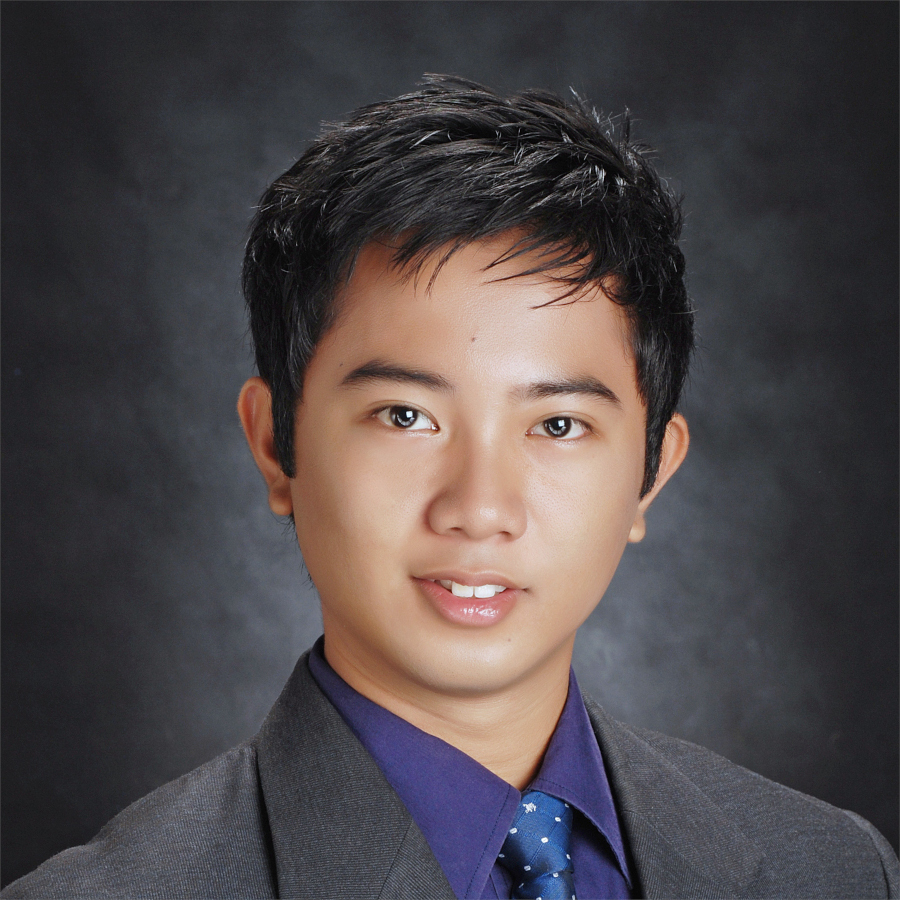
\includegraphics[width=1in]{img/rabi}} \\
    P-4, Magosilom, Cantilan, Surigao del Sur && \\
    ericbasil.rabi@gmail.com && \\
\end{tabularx}

\vspace{20pt}

\textbf{PERSONAL INFORMATION}

\vspace{-10pt}
\hrulefill

\begin{tabular}{@{}l@{ : }l}
    DATE OF BIRTH & January 17, 1991 \\
    PLACE OF BIRTH & Trinidad, Calbayog City, Samar \\
    AGE & 32 \\
    GENDER & Male \\
    NATIONALITY & Filipino \\
    RELIGION & Roman Catholic \\
    CIVIL STATUS & Married \\
    FATHER'S NAME & Ricardo A. Rabi \\
    MOTHER'S NAME & Ester C. Rabi \\
\end{tabular}

\vspace{20pt}

\textbf{EDUCATIONAL BACKGROUND}

\vspace{-10pt}
\hrulefill

\begin{tabular}{@{}l@{ : }l}
    COLLEGE & Saint Paul University Surigao \\
    & Corner Rizal and San Nicolas Streets, Surigao City \\
    HIGH SCHOOL & Philippine Science High School \\
    & Quezon City, Metro Manila \\
    ELEMENTARY & Trinidad Elementary School \\
    & Trinidad, Calbayog City, Samar \\
\end{tabular}

\newpage

\begin{tabularx}{\linewidth}{@{}lXr}
    \MakeUppercase{\authorb} && \multirow{3}{*}{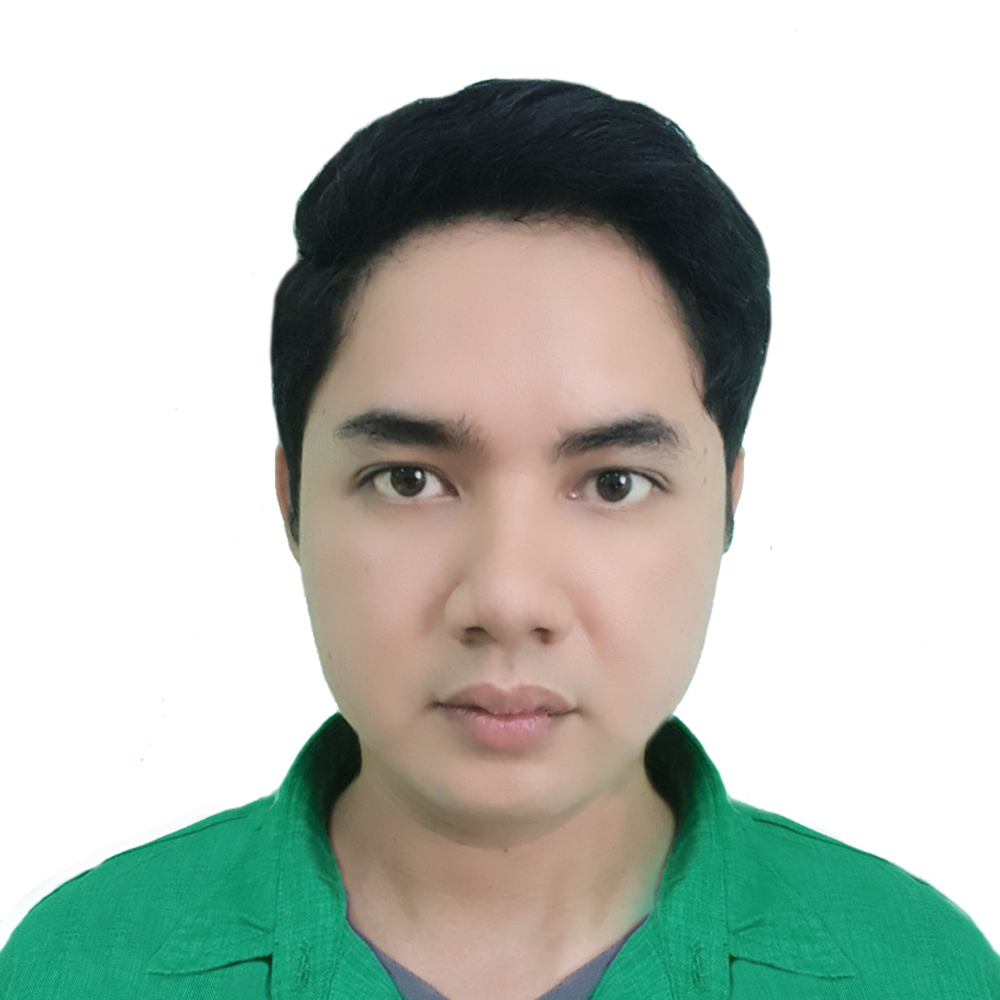
\includegraphics[width=1in]{img/James M.png}} \\
    Purok 1, Ladgaron, Claver, Surigao del Norte && \\
    xkitzie23@gmail.com && \\
\end{tabularx}

\vspace{20pt}

\textbf{PERSONAL INFORMATION}

\vspace{-10pt}
\hrulefill

\begin{tabular}{@{}l@{ : }l}
    DATE OF BIRTH & September 8, 1992 \\
    PLACE OF BIRTH & Pangi, Ladgaron, Claver, Surigao del Norte \\
    AGE & 30\\
    GENDER & Male \\
    NATIONALITY & Filipino \\
    RELIGION & Catholic\\
    CIVIL STATUS & Married \\
    FATHER'S NAME & Tomas N. Paje, Sr. \\
    MOTHER'S NAME & Luz M. Paje\\
\end{tabular}

\vspace{20pt}

\textbf{EDUCATIONAL BACKGROUND}

\vspace{-10pt}
\hrulefill

\begin{tabular}{@{}l@{ : }l}
    COLLEGE & Saint Paul University Surigao \\
    & Corner Rizal and San Nicolas Streets, Surigao City \\
    HIGH SCHOOL & Claver National High School \\
    & Tayaga, Claver, Surigao del Norte \\
    ELEMENTARY & Surigao West Central Elementary School \\
    & Brgy. San Juan, Surigao City \\
\end{tabular}

\newpage

\begin{tabularx}{\linewidth}{@{}lXr}
    \MakeUppercase{\authorc} && \multirow{3}{*}{
\includegraphics[width=1in]{img/velonta}} \\
    Blk. 5 Lot 9 Lopez Habitat, Brgy. Baan Km 3, Butuan City && \\
    jkvelonta@gmail.com && \\
\end{tabularx}

\vspace{20pt}

\textbf{PERSONAL INFORMATION}

\vspace{-10pt}
\hrulefill

\begin{tabular}{@{}l@{ : }l}
    DATE OF BIRTH & May 23, 1997 \\
    PLACE OF BIRTH & Butuan City\\
    AGE & 25\\
    GENDER & Male \\
    NATIONALITY & Filipino \\
    RELIGION & Scientology \\
    CIVIL STATUS & Single \\
    FATHER'S NAME & Greg S. Velonta\\
    MOTHER'S NAME & May C. Velonta\\
\end{tabular}

\vspace{20pt}

\textbf{EDUCATIONAL BACKGROUND}

\vspace{-10pt}
\hrulefill

\begin{tabular}{@{}l@{ : }l}
    COLLEGE & Saint Paul University Surigao \\
    & Corner Rizal and San Nicolas Streets, Surigao City \\
    HIGH SCHOOL & Philippine Science High School - Central Visayas Campus\\
    & Brgy. Talaytay, Argao, Cebu \\
    ELEMENTARY & Butuan Central Elementary School - Science and Technology Education Center \\
    & A.D. Curato Street, Butuan City \\
\end{tabular}

\newpage

\begin{tabularx}{\linewidth}{@{}lXr}
    \MakeUppercase{\authord} && \multirow{3}{*}{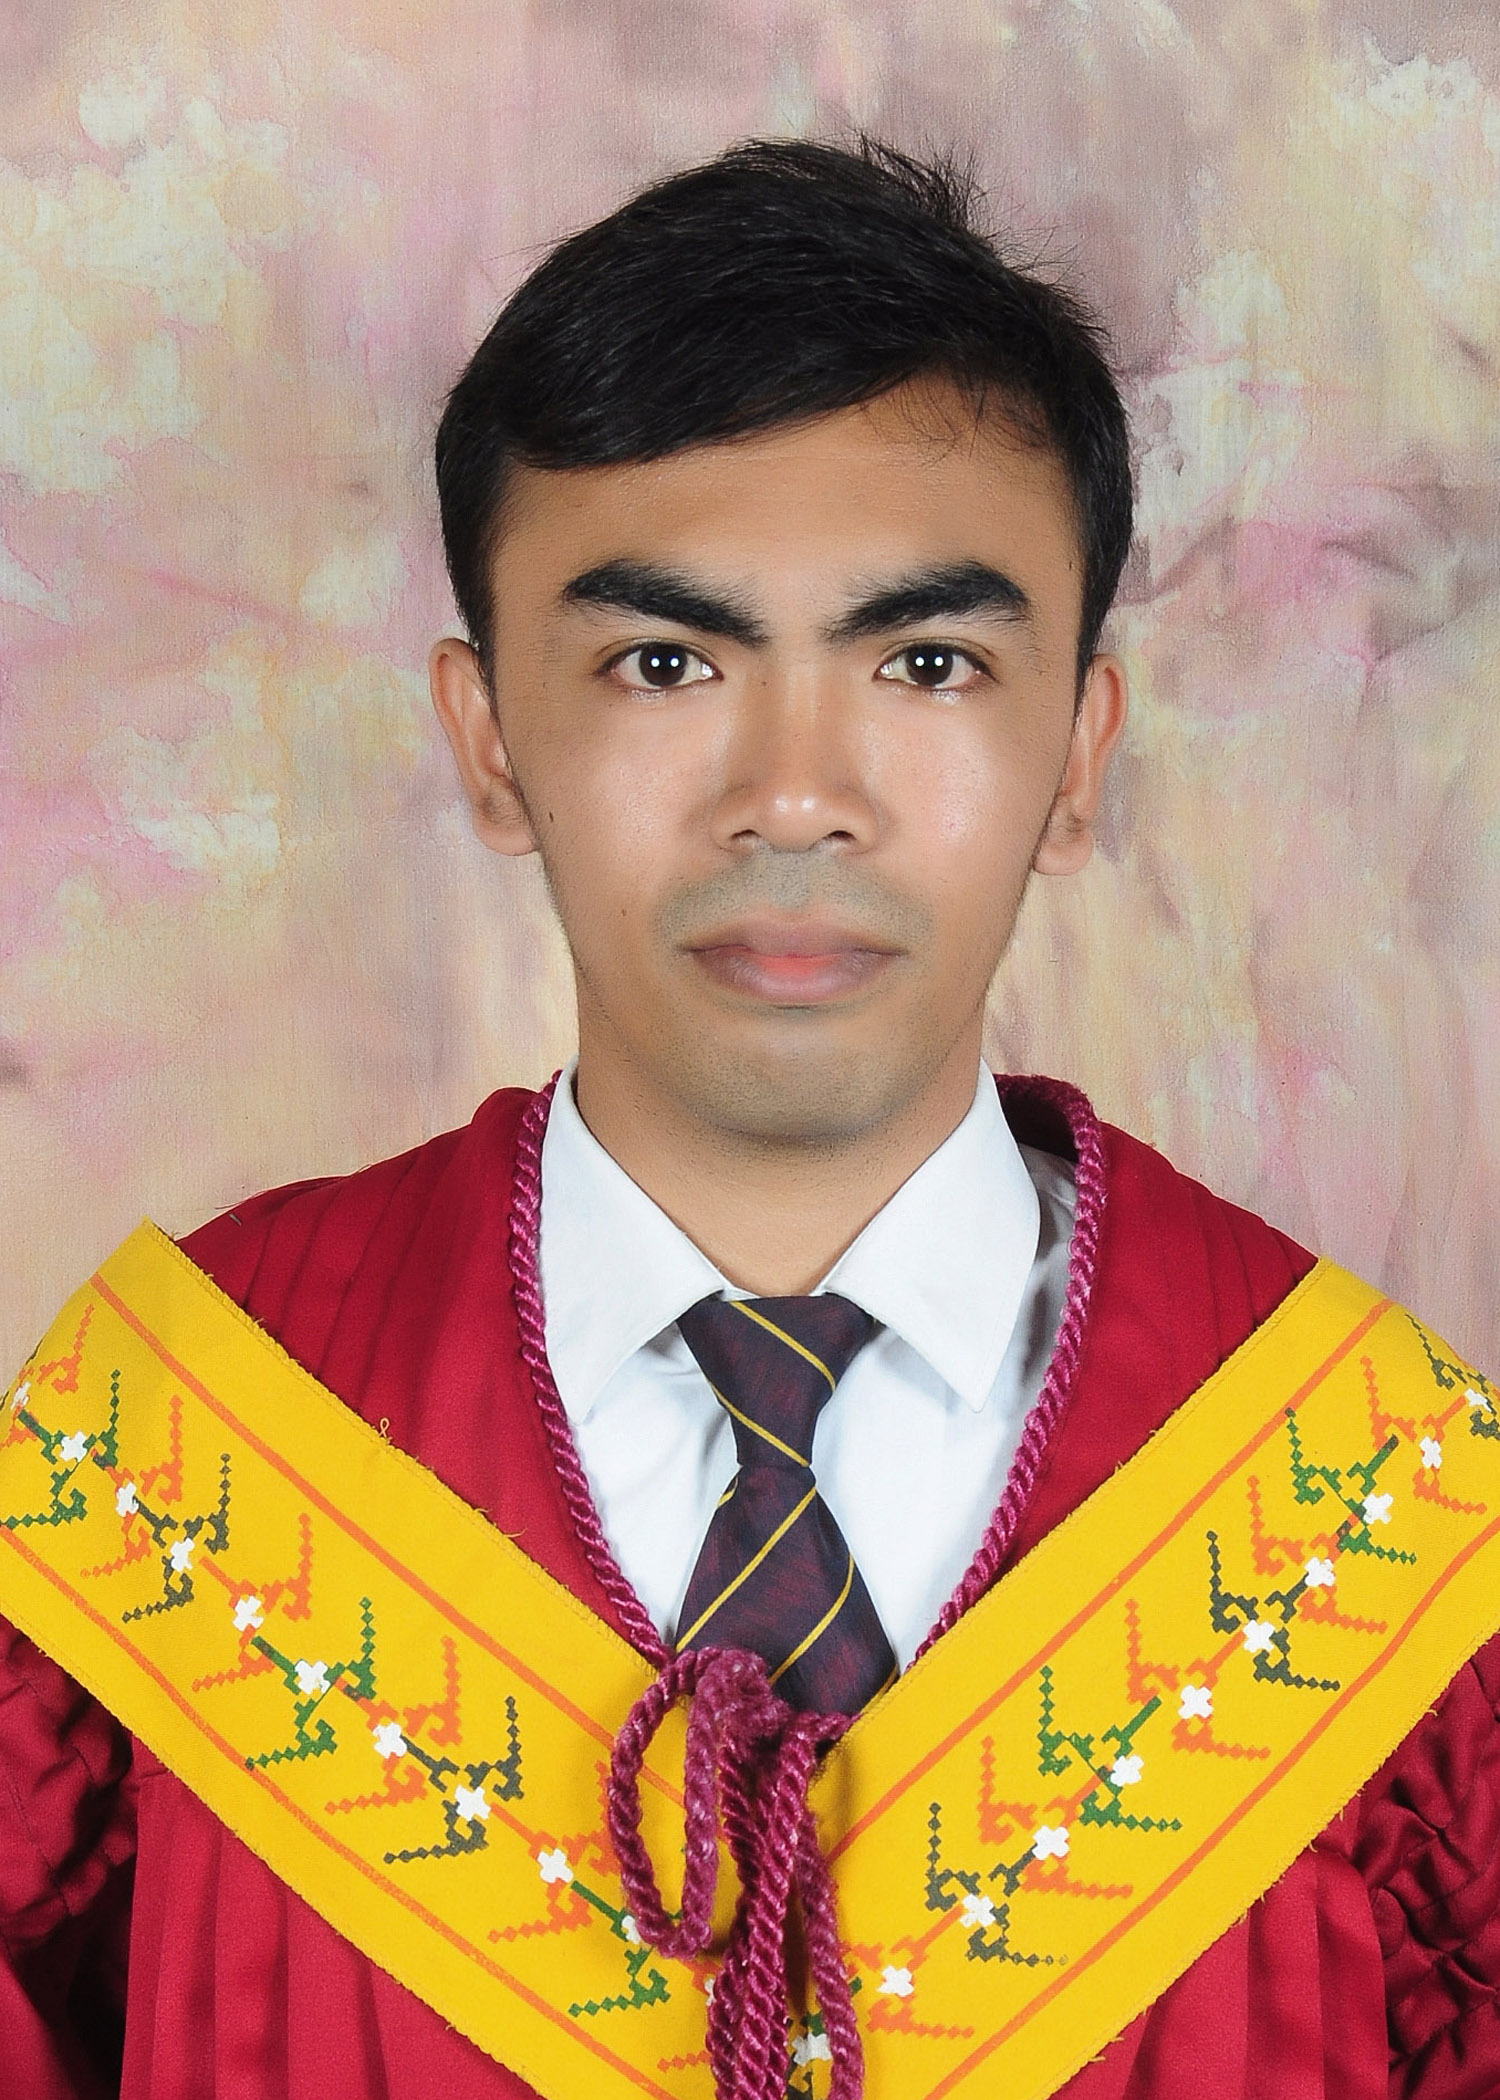
\includegraphics[width=1in]{img/banog}} \\
    Purok 6, Taganito, Claver, Surigao del Norte && \\
    richard.banog@mail.com && \\
\end{tabularx}

\vspace{20pt}

\textbf{PERSONAL INFORMATION}

\vspace{-10pt}
\hrulefill

\begin{tabular}{@{}l@{ : }l}
    DATE OF BIRTH & September 24,1990 \\
    PLACE OF BIRTH & Poblacion, Lingig, Surigao del Sur \\
    AGE & 32 \\
    GENDER & Male \\
    NATIONALITY & Filipino \\
    RELIGION & Iglesia ni Cristo \\
    CIVIL STATUS & Single  \\
    FATHER'S NAME & N/A \\
    MOTHER'S NAME &  Norita Maganyan Banog\\
\end{tabular}

\vspace{20pt}

\textbf{EDUCATIONAL BACKGROUND}

\vspace{-10pt}
\hrulefill

\begin{tabular}{@{}l@{ : }l}
    COLLEGE & Saint Paul University Surigao \\
    & Corner Rizal and San Nicolas Streets, Surigao City \\
    HIGH SCHOOL & Lingig National High School \\
    & Poblacion, Lingig, Surigao del Sur \\
    ELEMENTARY & Hinipaan Elementary School \\
    & Hinipaan, Poblacion, Lingig, Surigao del Sur \\
\end{tabular}

\end{spacing}
\end{document}
